\documentclass[letterpaper, 11pt]{article}
\usepackage[margin=1in]{geometry}

\usepackage[autostyle, english=american]{csquotes}
\MakeOuterQuote{"}

\usepackage{hyperref}
\usepackage[]{algorithm2e}
\usepackage{multirow}
\usepackage{subfig}
\usepackage{graphicx}
\graphicspath{ {../} }
\usepackage{float}

\usepackage{biblatex-chicago}
\addbibresource{references.bib}
\pdfgentounicode=1


\title{Risk Aversion and Gender in Chess}
\author{Charlie Mayville}

\begin{document}
\maketitle

    \begin{abstract}
        This paper aims to use double ML estimators to measure the direct casual effect of gender on risk behavior in chess players.
        Features of modern chess engines allow for precise and relatively unbiased measurement of the risk for particular chess moves.
        In contrast to previous literature, we find a small causal effect indicating less risk aversion in female identifying chess players.
    \end{abstract}

    \section*{Introduction}
        The effect of gender on risk aversion is often studied in economics, and the popular and controversial claim is that women are on average more risk averse and less competitive than men.
        Chess provides a unique opportunity to study this effect, as it is extensively well documented, and has an objective measure of skill: Elo rating.
        Gerdes and Gränsmark\footcite{gerdes:gender} attempted to measure the direct causal effect of gender on risk taking in chess in 2010.
        They found that, in line with related literature, female chess players were to a small extent more risk averse than their male counterparts.
    
        In this paper, we follow their analysis, changing two main things. 
        First, we use features of modern chess engines to compute a more wholistic and objective measurement of risk taking behavior. 
        Second, we relax their parametric assumptions and instead measure the direct casual effect with a double robust estimator.
        
        We find a small but significant causal effect pointing in the opposite direction of previous literature---women are on average more risk taking in our analysis then men.

    \section*{Model}
        The direct causal effect of gender on risk aversion can be represented as the average treatment effect (ATE), or the difference between the risk aversion of a player and the same player in a world where only their gender was changed.
        Formally:
        $$ ATE = E[ Y | do( A = 1) ] - E[ Y | do ( A = 0) ] $$
        Where $Y$ is some measure of risk aversion and $A$ is an indicator for gender.
    
    \subsection*{Ordinary Least Squares}
        
        The authors of the original paper use ordinary least squares in the following linear probability model (LPM) to estimate the causal effect of gender on risk aversion. For player $i$:
        $$Y_{ij} = \alpha_{ij} + \beta A_{i} + X_{ij} \pi + e_{ij}$$
        where $A_i$ is the indicator for gender, and $X_{ij}$ is a set of confounders including age, Elo rating, region\footnote{a rough categorization of player nationality}, and number of games.

        Not only does this model make heavy handed parametric assumptions in order to estimate the ATE, but it lacks interaction terms and utilizes a frightenly small number of covariates.
        Notably missing are whether or not a player is titled---a factor that reduces potential losses in rating and perceived status---and K-factor, which measures the amount of rating points at stake in a particular game. 

    \subsection*{AIPTW}
        
        Rather than resorting to parametric assumptions, we can find a double robust estimate of the average treatment effect with just two important assumptions:
        \begin{enumerate}
        \item \emph{No Un-observed Confounders}\\
              In other words the set of confounders we measure is the only set of confounders that effect risk aversion. Our confidence in this assumption can be calculated for any model we fit.
        \item \emph{Overlap}\\
              That is $\forall x$ : $ 0 < P( A = 1 | X = x ) < 1 $ \\
              This assumption is testable for any model we fit to the estimator.
        \end{enumerate}

        With both these assumptions made we can estimate the average treatment effect with a standard double robust model:
        $$ \hat{\tau}^{AIPTW} = \frac{1}{n} \sum_i \hat{Q}(1, X_i) - \hat{Q}(0, X_i) + A_i \frac{Y_i - \hat{Q}(1, X_i)}{\hat{g}(X_i)} - ( 1 - A_i ) \frac{Y_i - \hat{Q}(0, X_i)}{\hat{g}(X_i)} $$
        Which is not reliant on mutual robustness of either $\hat{Q}$ or $\hat{g}$, our estimated functions for the conditional expected outcome, and the propensity score respectively. 

    \subsection*{Risk Aversion}
        Gerdes and Gränsmark attempt to measure the risk taking demonstrated in a particular chess game by qualitatively analizing the opening position of each game.
        A list of openings were submitted to a panel of chess experts, who categorized them into "risky" and "solid" openings.
        A player's individual game's risk aversion was then scored based on its first few moves.

        This approach has a couple of problems. 
        First, most of each game is not played in the opening.
        While it can be argued that certain openings almost always lead to risky or risk averse situations (take the Grünfeld for example) the vast majority of openings are hardly deterministic in the risk level of the following play.
        Second, with a small sample size of individual players, it is impossible to completely eliminate the risk of personal bias or lack of understanding of particular positions. We propose measuring risk aversion with the use of a chess engine.

        Since 2010, advances in chess computers have opened up a more wholistic and objective way to measure risk.
        When we refer to risky behavior in chess, we usually mean playing towards positions that increase the variability in outcome.
        Holding equal for the quality of move, some function of reduction in the probability of a draw would be a good estimate for risk prone play.
        Modern chess engines that run on neural networks utilize a kind of chess evaluation called win draw loss (WDL), where a position is evaluated not on the amount of effective material present, but on the position's perceived winning chance.

        Utilizing the ability to calculate WDL gives us a percentage likelihood of the game resulting in a win, draw or loss, which we use in the following algorithm to calculate a players risk score in a given game: \\ \\ 
        \begin{algorithm}[H]
            previous win, draw, loss $\gets$ evaluate( initial position )\;
            \For{player's move in game}{
                make move\;
                current win, draw, loss $\gets$ evaluate( position )\;
                \eIf{ abs(previous win - current win) $<$ abs(previous loss - current loss) }{
                    score $\gets$ previous win - current win\;
                }{
                    score $\gets$ previous loss - current loss\;
                }
                add score to scores\;
            }
            find average of scores\;
        \end{algorithm}
        \hfill \break
        \noindent In practice\footnote{running on Leela Chess Zero version 0.28 with the standard provided 5G network file\\ (7ca2381cfeac5c280f304e7027ffbea1b7d87474672e5d6fb16d5cd881640e04)}, these scores ranged from about 100 to 200, and higher scores indicate riskier play. 
        Risk scores were then averaged across each game to create on metric per player.


    \section*{Data and Statistics}
        The data for the analysis was collected from two sources.
        The World Chess Federation, or \emph{FIDE}, keeps a publicly available list of active players\footcite{fide-ratings}, numbering well over 400,000.
        Game specific data was drawn from ChessTempo\footcite{chesstempo}, a freely available database containing over 3 million games.

        To reduce potential inaccuracies with estimating a players strength and playstyle over an extended period of time, games were collected within the span of one year---2019.\footnote{The year 2019 was chosen since it is the most recent year without a significant effect of COVID lockdowns on games, when many official tournaments moved online and adopted marginally different rulesets.}
        We found wild variations in a players risk score when analysing less than ten games. 
        In order to accurately measure a players average risk score we further limited the dataset to those players with 20 or more games in 2019.
        In total we were able to analyze over 200,000 games spread out over 4108 distinct players, 3467 men and 641 women.

    \subsection*{Model Fitting}
        We fit several models on the data with 10 folds, and calculated their cross validated mean squared error. 
        Each model included Elo rating, nationality, title, K-factor, age, number of recorded games played in 2019, and the players average opponent rating as confounders.
        The following table shows each models error and the baseline error of the data: \\

        \begin{tabular}{ |p{4cm}||p{2cm}|p{2cm}|p{3cm}|p{3cm}| }
            \hline
            \multicolumn{5}{|c|}{Model Fit Diagnostics} \\
            \hline
            model & $\hat{Q}$ mse & $\hat{g}$ ce & baseline mse & baseline ce\\
            \hline
            RF (depth = max) & 9.063 & 0.309 & 9.747 & 0.432 \\
            RF (depth = 10)  & 8.681 & 0.310 & 9.747 & 0.432 \\
            XGB              & 10.00 & 0.324 & 9.747 & 0.432 \\
            Lin/Log          & 8.611 & 0.376 & 9.747 & 0.432 \\
            \hline
        \end{tabular} \\

        Each estimator does at least a good enough job to be better than the error with no fit, except XGBoost, which is a particularly bad estimator of $Q$.
        Interestingly enough, the linear model served as one of the best estimators of conditional outcome, perhaps because of the high amount of data relative to the number of confounders.

    \subsection*{Overlap Assumptions}

        In order to satisfy the overlap assumption for our estimator of the ATE, we need the propensity scores to be strictly less than one and greater than zero for all $x \in X$. 
        Looking at Figure 1, that assumption is easily met for all our models:

        \begin{figure}[H]
            \centering
            \subfloat{{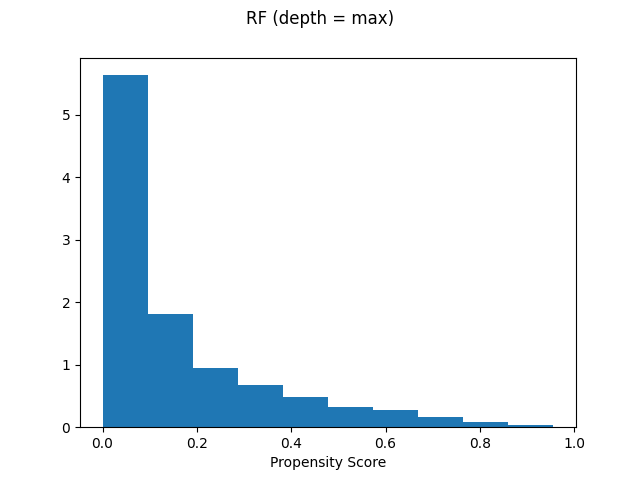
\includegraphics[width=3.7cm]{RF (depth = max).png} }}
            \quad
            \subfloat{{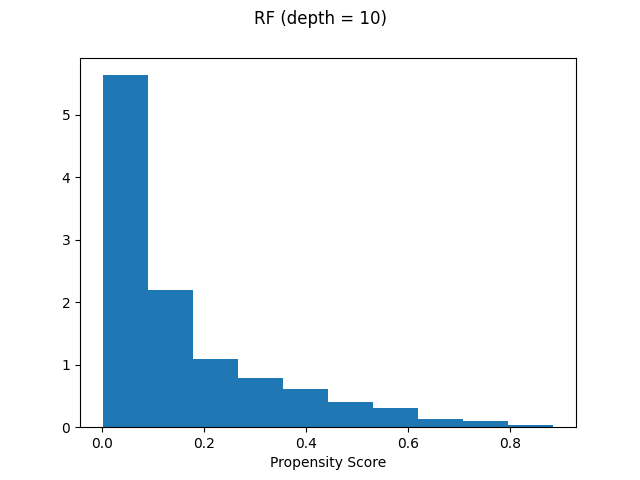
\includegraphics[width=3.7cm]{RF (depth = 10).png} }}
            \quad
            \subfloat{{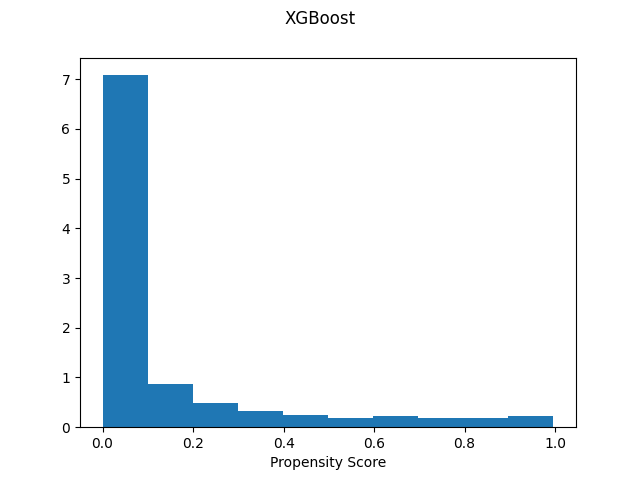
\includegraphics[width=3.7cm]{XGBoost.png} }}
            \quad
            \subfloat{{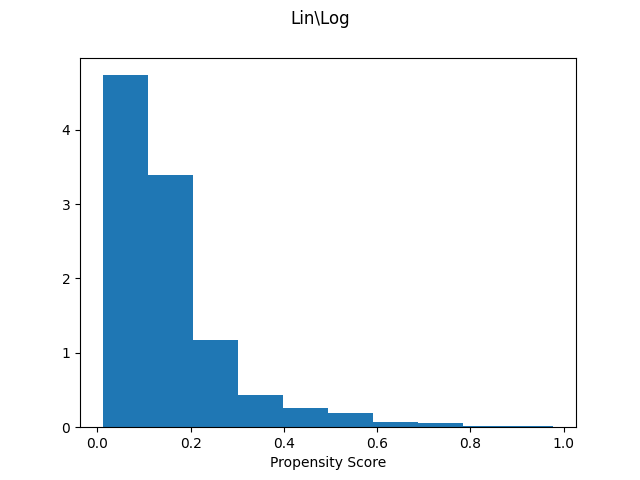
\includegraphics[width=3.7cm]{Lin-Log.png} }}
            \caption{Propensity Scores}
            \label{fig:example}
        \end{figure}

    \subsection*{ATE estimation}

        We can plug in our estimated $\hat{Q}$ and $\hat{g}$'s into our $AIPTW$ estimate for the average treatment effect.
        A positive effect indicates riskier play in women.
        Constructing 95\% confidence intervals we see that the only model with a significant estimate is linear.\footnote{How tragic!} \\

        {
        \centering
        \begin{tabular}{ |p{4cm}||p{2cm}|p{2cm}| }
            \hline
            \multicolumn{3}{|c|}{Confidence Interval of ATE} \\
            \hline
            model & estimate & + / - \\
            \hline
            RF (depth = max) & 1.091 & 1.429 \\
            RF (depth = 10)  & 1.966 & 2.509 \\
            Lin/Log          & 0.790 & 0.348 \\
            \hline
        \end{tabular} \par
        }

    \subsection*{Sensitivity Analysis}
        
        In addition to overlap, our other assumption is that we had no unobserved confounders.
        We can quickly test the effect such an unobserved confounder might have by fitting the same model to the data again, dropping one observed confounder and measuring the change in our estimate.
        
        \begin{figure}[H]
            \centering
            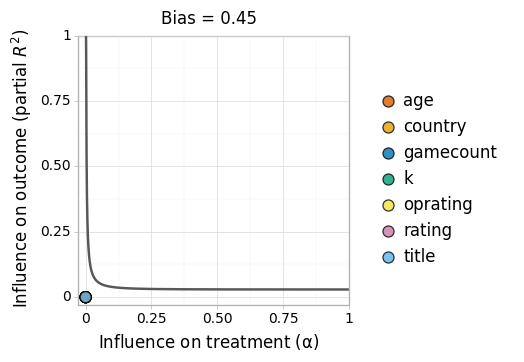
\includegraphics[width=7cm]{austen_plot.png}
            \caption{Austen Plot}
        \end{figure} 

        The resulting Austen plot provides little reason to suspect that an unobserved confounder could have enough effect to render our result non-significant.

    \section*{Conclusion}
        
        We see a significant causal effect of gender on risk aversion in chess---indicating less risk aversion in female identifying players---in the neighborhood of half a percentage point.
        Testing our assumptions, we have no immediate reason to assume a ill-crafted estimate.
        However, due to the small number of covariates observed, the complicated nature of such an effect, and the number of model classes which failed, we would suggest caution in interpreting such results.
        Perhaps a closer look at fewer players could provide a more convincing analysis.

    \subsection*{Code}
        
        Code is available at \href{https://github.com/cmayville/chess-gender-risk}{github.com/cmayville/chess-gender-risk}.



        



\nocite{lc0}
\newpage
\printbibliography
\end{document}

